\begin{frame}{ReAct}
  \begin{itemize}
    \item ReAct is a framework where LLMs are used to generate both reasoning traces and task-specific actions in an interleaved manner
    \begin{itemize}
      \item \textbf{Generating reasoning traces} allow the model to induce, track, and update action plans, and even handle exceptions
      \item \textbf{The action step} allows to interface with and gather information from external sources such as knowledge bases or environments.
    \end{itemize}
    \item ReAct allows LLMs to interact with external tools to retrieve additional information that leads to more reliable and factual responses
  \end{itemize}
  \vfill
  {\scriptsize
    \color{gray!75!black}
    Source: Yao et al., ``ReAct: Synergizing Reasoning and Acting in Language Models'', ICLR 2023, \url{https://arxiv.org/abs/2210.03629}
  }
\end{frame}

\begin{frame}{ReAct Example}
  \centering
  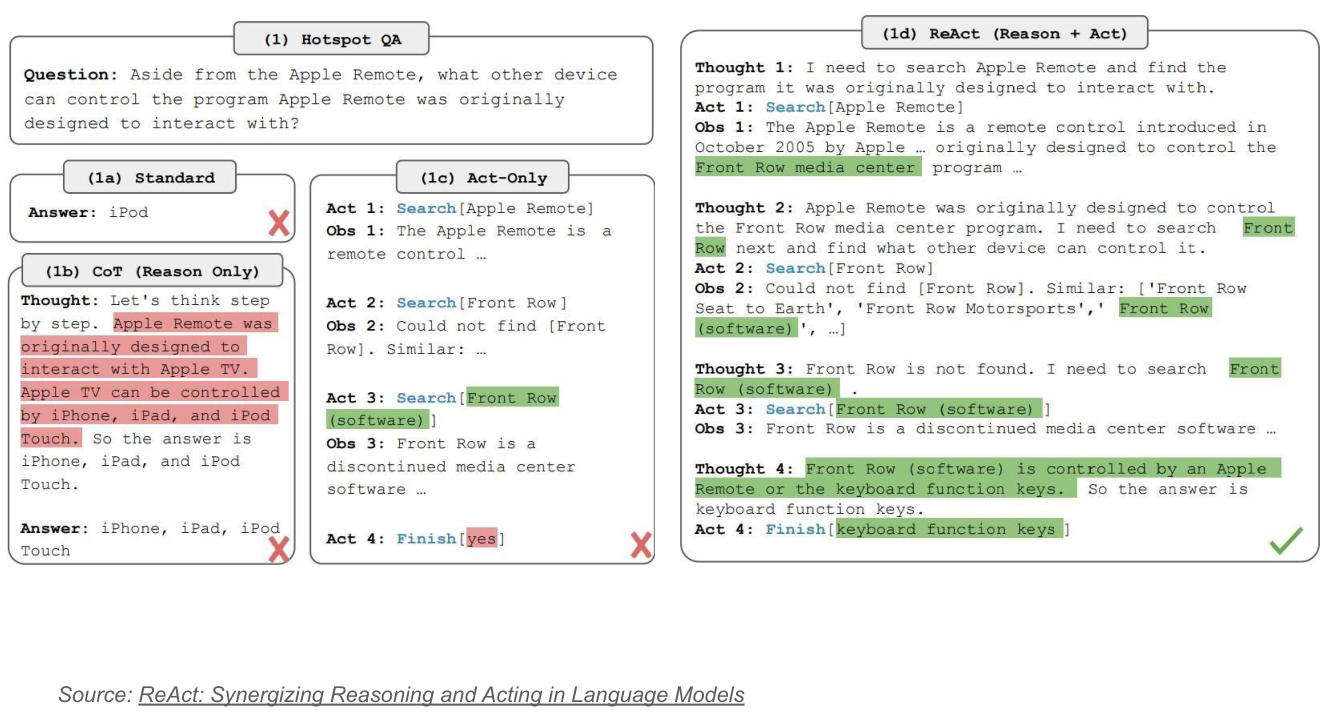
\includegraphics[width=0.9\textwidth, height=0.82\textheight, keepaspectratio]{images/prompting-rag/prompting_react_reasoning_acting_comparison.png}

  {\scriptsize
    \color{gray!75!black}
    Source: Yao et al., ICLR 2023, \url{https://arxiv.org/abs/2210.03629}
  }
\end{frame}
